\documentclass[10pt]{beamer}
\usepackage[english]{babel}
\usepackage[utf8]{inputenc}
\usepackage[T1]{fontenc}
\usepackage{helvet}


%-------------------------------------------------------
% INFORMATION IN THE TITLE PAGE
%-------------------------------------------------------

\newcommand{\cstitle}{\textbf{Bioinformatics against COVID-19}}
\subtitle[]{Research Group in Bioinformatics}
\newcommand{\cscourseCode}{1005155}
\newcommand{\csauthor}{MSc. Vicente Machaca Arceda}
%\institute[UNSA]{Universidad Nacional de San Agustín de Arequipa}
\newcommand{\csemail}{vmachacaa@unsa.edu.pe}
\newcommand{\instituteabr}{UNSA}
\newcommand{\nameUp}{ICC Fase 1}
\date{\today}
\title[\cscourseCode]{\cstitle}
\author{\csauthor}
%%%%%%%%%%%%%%%%%

%-------------------------------------------------------
% CHOOSE THE THEME
%-------------------------------------------------------
\def\mycmd{0} % CS THEME
\def\mycmd{1} % MYTHEME
%-------------------------------------------------------

\if\mycmd1
	\usetheme[]{Feather}
	\newcommand{\chref}[2]{	\href{#1}{{\usebeamercolor[bg]{Feather}#2}} }
\else
	\usepackage{csformat}
\fi

\newcommand{\1}{
        	\setbeamertemplate{background}{
        		
\includegraphics[width=\paperwidth,height=\paperheight]{img/1}
        		\tikz[overlay] \fill[fill opacity=0.75,fill=white] (0,0) rectangle (-\paperwidth,\paperheight);
        	}
}



%-------------------------------------------------------
% THE BODY OF THE PRESENTATION
%-------------------------------------------------------

\begin{document}


\AtBeginSubsection[]
{
    \begin{frame}
        \frametitle{Table of Contents}
        \tableofcontents[currentsubsection]
    \end{frame}
}


%-------------------------------------------------------
% THE TITLEPAGE
%-------------------------------------------------------

\if\mycmd1 % MY THEME
	\1{
	\begin{frame}[plain,noframenumbering] 
		\titlepage 
	\end{frame}}

\else % CS THEME
	\maketitle
\fi


%-------------------------------------------------------
%-------------------------------------------------------
\begin{frame}{Overview}
	\tableofcontents
\end{frame}
%-------------------------------------------------------
%-------------------------------------------------------


\section{Introduction}

%%%%%%%%%%%%%%%%%%%%%%%%%%%%%%%%%%%%%%%%%%%%%%%%%%%%%%%%
\subsection{Objectives}
%%%%%%%%%%%%%%%%%%%%%%%%%%%%%%%%%%%%%%%%%%%%%%%%%%%%%%%%

%-------------------------------------------------------
%-------------------------------------------------------
\begin{frame}{Objectives}{}
	\begin{itemize}
		\item<1-> Understand what is Bioinformatics. 
		\item<2-> Learn areas of research of Bioinformatics related to COVID-19.
	\end{itemize}
\end{frame}
%-------------------------------------------------------
%-------------------------------------------------------


%%%%%%%%%%%%%%%%%%%%%%%%%%%%%%%%%%%%%%%%%%%%%%%%%%%%%%%%
\subsection{Presentation}
%%%%%%%%%%%%%%%%%%%%%%%%%%%%%%%%%%%%%%%%%%%%%%%%%%%%%%%%

%-------------------------------------------------------
%-------------------------------------------------------
\begin{frame}{Presentation}{}
	\begin{itemize}
		\item<1-> MSc. Vicente Enrique Machaca Arceda. 
		\item<2-> Professor at UNSA university.
		\item<3-> Full time researcher at La Salle university.		
		\item<4-> Leader of research group of Bioinformatics in Arequipa.
	\end{itemize}
\end{frame}
%-------------------------------------------------------
%-------------------------------------------------------

%-------------------------------------------------------
%-------------------------------------------------------
\begin{frame}{Presentation}{Publications}
	\begin{table}[]
		\setlength{\tabcolsep}{0.5em} % for the horizontal padding
		{\renewcommand{\arraystretch}{1.4}% for the vertical padding
		\begin{tabular}{llp{7cm}}
			\textbf{Year} & \textbf{Country} & \textbf{Title}                                                                                                              \\
			\hline
		
			2018          & Brasil           & Fast Car Crash Detection in Video                                                                                           \\
			2016          & Chile            & Fast Face Detection in Violent Video Scenes                                                                                 \\
			2016          & Costa Rica       & Real Time Violence Detection in Video with ViF and Horn-Schunck                                                             \\
			2016          & Costa Rica       & Optimization model for face detection in video sequences                                                                    \\
			2015          & Chile            & Real Time Violence Detection in Video                                                                                      
		\end{tabular}
	}
	\end{table}
\end{frame}
%-------------------------------------------------------
%-------------------------------------------------------

%-------------------------------------------------------
%-------------------------------------------------------
\begin{frame}{Presentation}{Publications}
	\begin{table}[]
		\setlength{\tabcolsep}{0.5em} % for the horizontal padding
		{\renewcommand{\arraystretch}{1.4}% for the vertical padding
		\begin{tabular}{llp{8cm}}
			\textbf{Year} & \textbf{Country} & \textbf{Title}                                                                                                              \\
			\hline
			2020          &                  & DNA sequence similarity analysis using Chaos Game Representation                                                            \\
			2020          &                  & Machine Learning and Chaos Game Representation for rapid classification of novel pathogens COVID-19 case study              \\
			2020          & Canada           & An analysis of k-mer frequency features with machine learning models for viral subtyping of  Polyomavirus and HIV-1 genomes \\
			2020          & Canada           & Forecasting time series with Multiplicative Trend Exponential Smoothing and LSTM: COVID-19 case study                       \\
			2020          & USA              & Small Ship Detection on Optical Satellite Imagery with YOLO and YOLT                                                        \\
			                       
		\end{tabular}
	}
	\end{table}
\end{frame}
%-------------------------------------------------------
%-------------------------------------------------------

%%%%%%%%%%%%%%%%%%%%%%%%%%%%%%%%%%%%%%%%%%%%%%%%%%%%%%%%
\subsection{The purpose of Bioinformatics}
%%%%%%%%%%%%%%%%%%%%%%%%%%%%%%%%%%%%%%%%%%%%%%%%%%%%%%%%


%-------------------------------------------------------
%-------------------------------------------------------
\begin{frame}{The purpose of Bioinformatics}{Why a person has cancer?}
	\begin{figure}[]
		\centering
		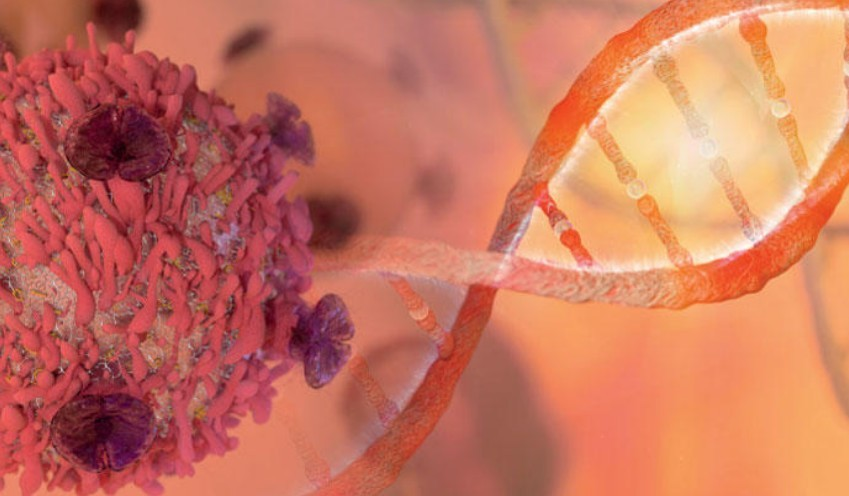
\includegraphics[width=\textwidth,height=0.6\textheight,keepaspectratio]{img/introduction/mot3.jpg}
		\label{img:mot2}
		\caption{Why a person has cancer?}
	\end{figure}
\end{frame}
%-------------------------------------------------------
%-------------------------------------------------------

%-------------------------------------------------------
%-------------------------------------------------------
\begin{frame}{The purpose of Bioinformatics}{Why some medicines no work in some persons?}
	\begin{figure}[]
		\centering
		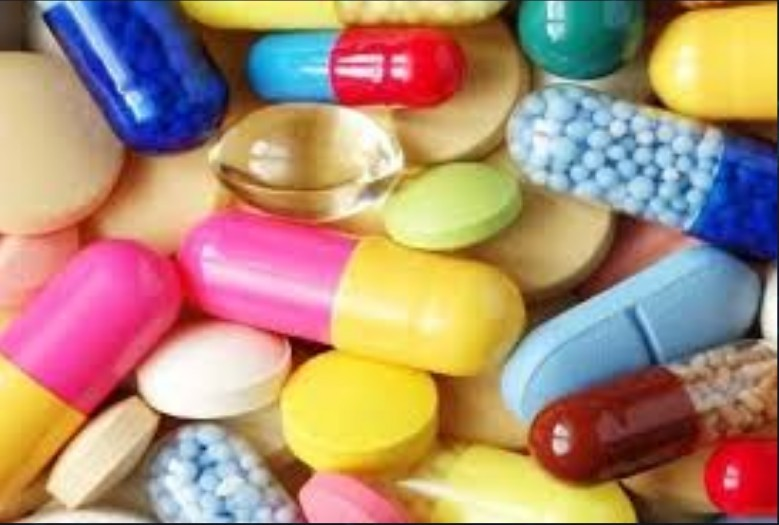
\includegraphics[width=\textwidth,height=0.6\textheight,keepaspectratio]{img/introduction/mot4.jpg}
		\label{img:mot2}
		\caption{Why some medicines no work in some persons?}
	\end{figure}
\end{frame}
%-------------------------------------------------------
%-------------------------------------------------------

%-------------------------------------------------------
%-------------------------------------------------------
\begin{frame}{The purpose of Bioinformatics}{Treatment Development}
	\begin{figure}[]
		\centering
		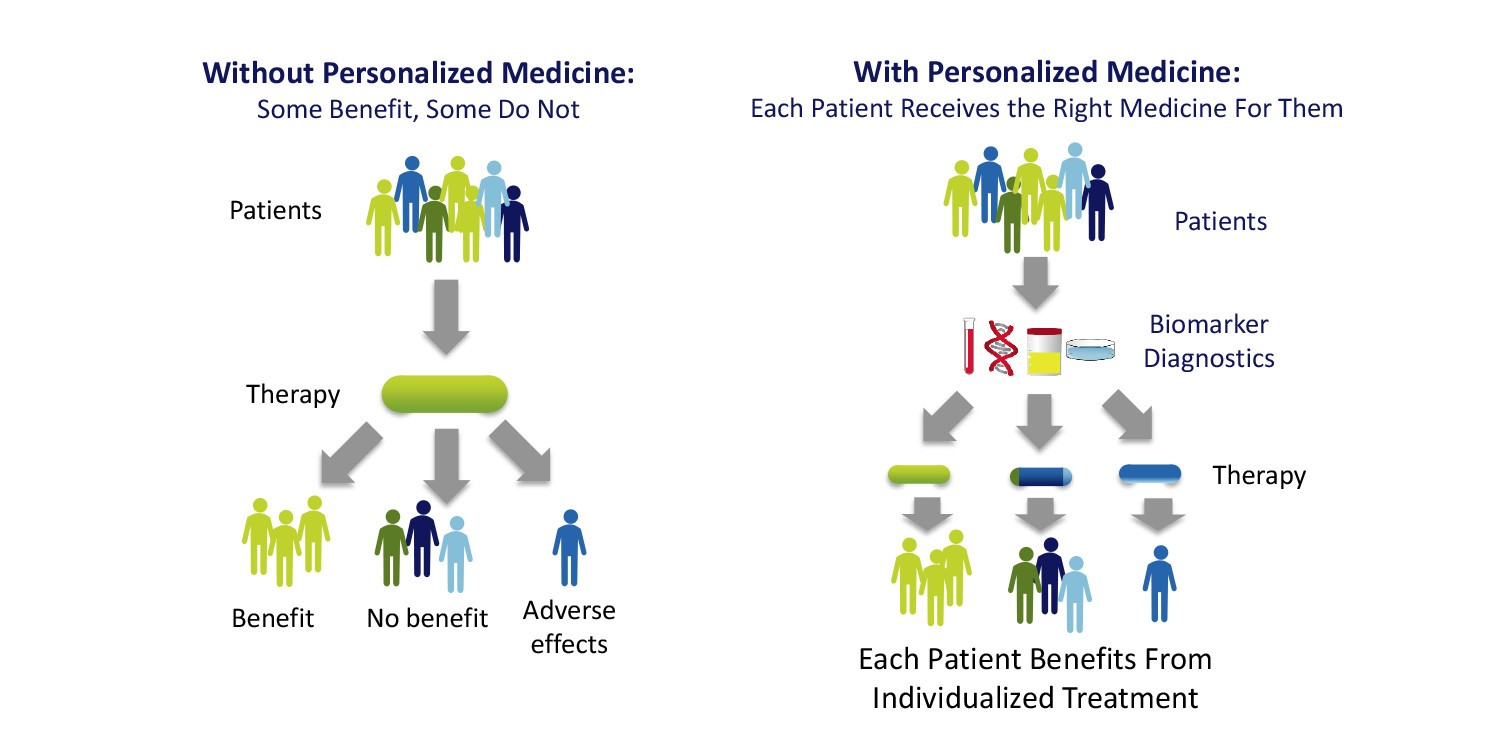
\includegraphics[width=\textwidth,height=0.7\textheight,keepaspectratio]{img/introduction/mot5.jpg}
		\label{img:mot2}
		\caption{Personalized Medicine: New Approach to Treatment of Disease}
	\end{figure}
\end{frame}
%-------------------------------------------------------
%-------------------------------------------------------

%-------------------------------------------------------
%-------------------------------------------------------
\begin{frame}{The purpose of Bioinformatics}{Protein simulation}
	\begin{figure}[]
		\centering
		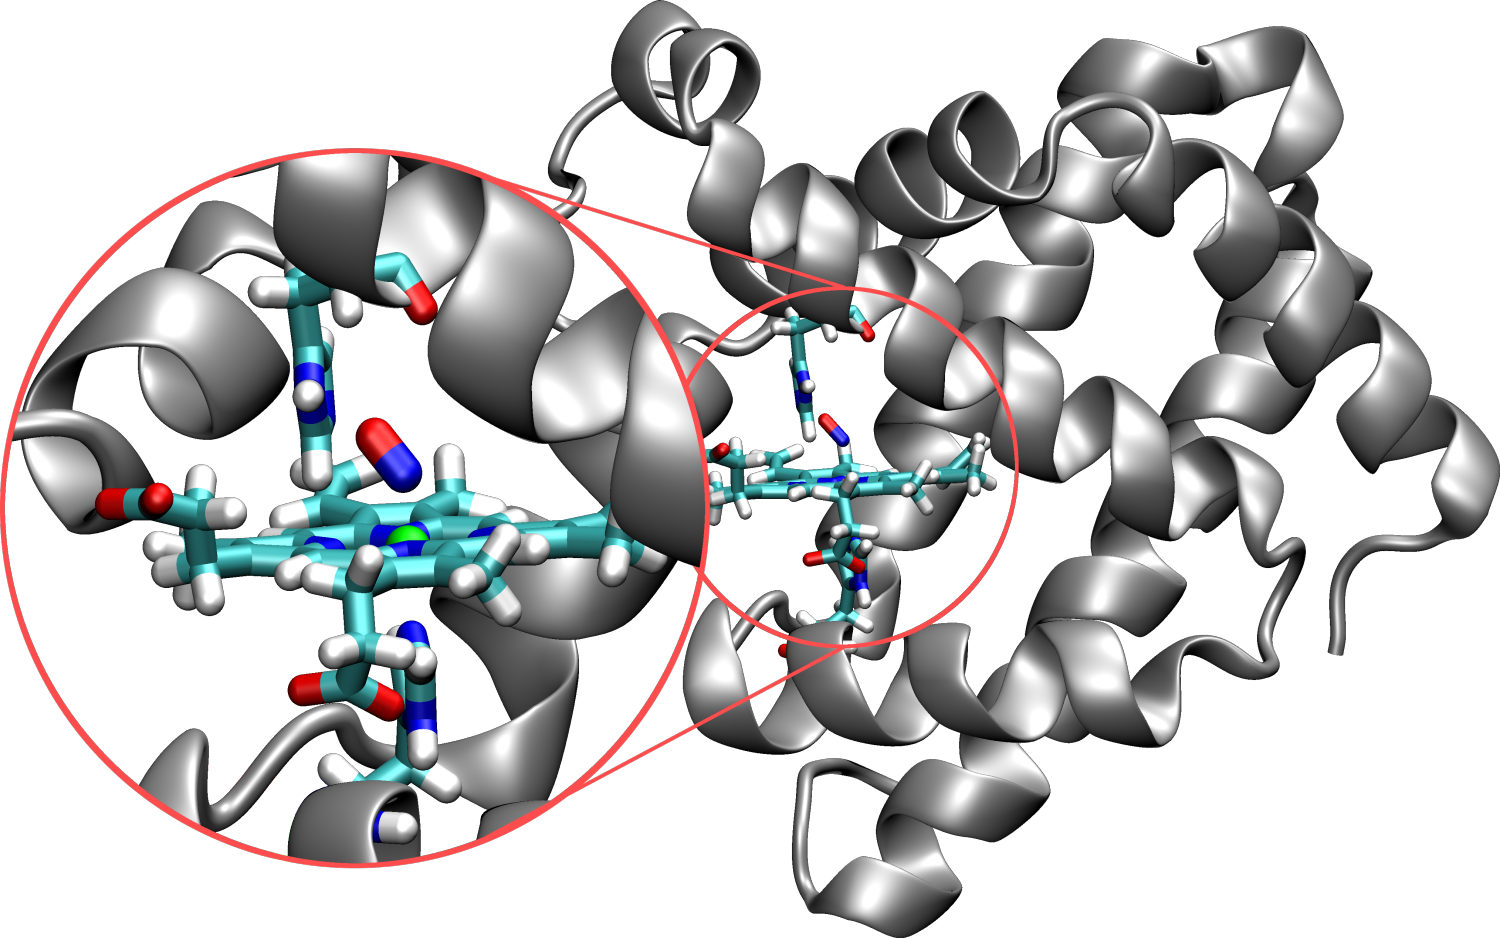
\includegraphics[width=\textwidth,height=0.7\textheight,keepaspectratio]{img/webinar/protein2}
		%https://www.pngwing.com/en/free-png-mrxlb
		\label{img:mot2}
		\caption{Computer simulation of protein-ligand.}
	\end{figure}
\end{frame}
%-------------------------------------------------------
%-------------------------------------------------------



%%%%%%%%%%%%%%%%%%%%%%%%%%%%%%%%%%%%%%%%%%%%%%%%%%%%%%%%
\subsection{What is Bioinformatics?}
%%%%%%%%%%%%%%%%%%%%%%%%%%%%%%%%%%%%%%%%%%%%%%%%%%%%%%%%

%-------------------------------------------------------
%-------------------------------------------------------
\begin{frame}{Introduction}{What is Bioinformatics?}
	
	According to Luscombe et al.: \textbf{Bioinformatics} involves the technology that uses computers for storage, retrieval, manipulation, and distribution of information related to biological macromolecules such as DNA, RNA, and proteins \cite{luscombe2001bioinformatics}.
	
\end{frame}
%-------------------------------------------------------
%-------------------------------------------------------



%-------------------------------------------------------
%-------------------------------------------------------
\begin{frame}{Bioinformatics}
	\begin{figure}[]
		\centering
		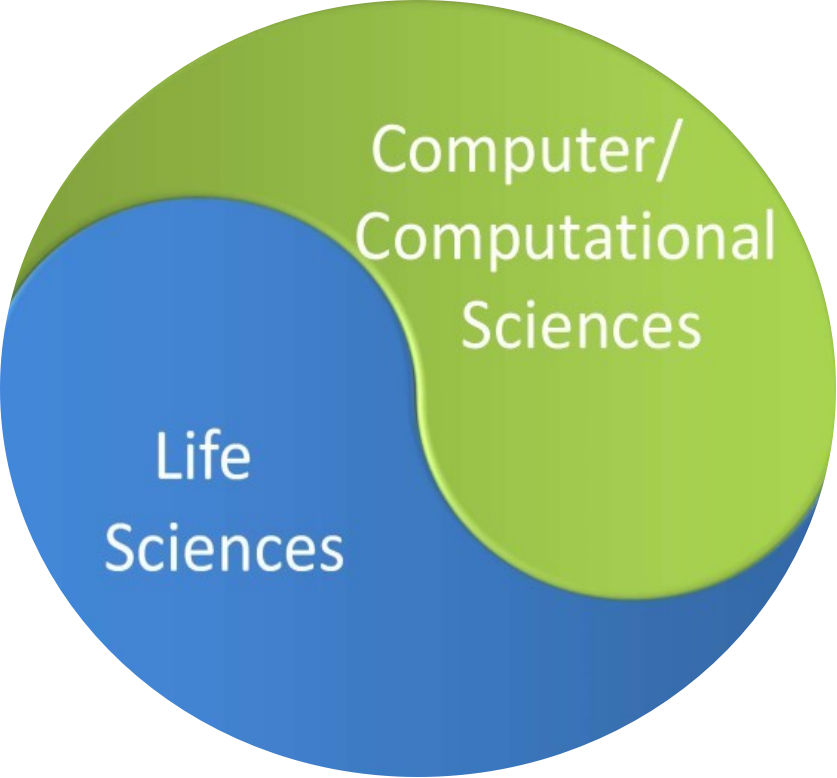
\includegraphics[width=\textwidth,height=0.7\textheight,keepaspectratio]{img/webinar/bio2.png}
		\label{img:mot2}
		%\caption{Computer simulation of protein-ligand.}
	\end{figure}
\end{frame}
%-------------------------------------------------------
%-------------------------------------------------------


%-------------------------------------------------------
%-------------------------------------------------------
\begin{frame}{Bioinformatics}
	\begin{figure}[]
		\centering
		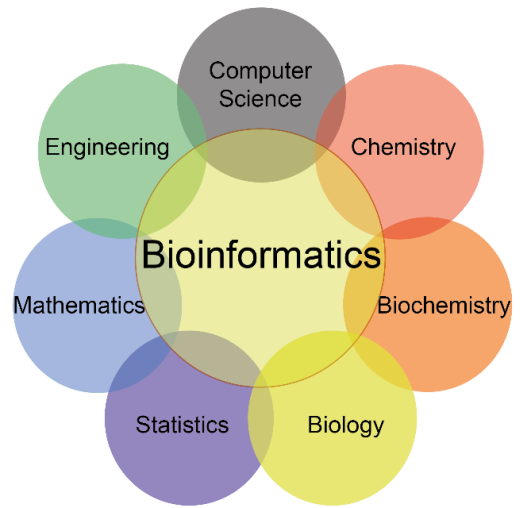
\includegraphics[width=\textwidth,height=0.7\textheight,keepaspectratio]{img/webinar/bio4}
		\label{img:mot2}
		%\caption{Computer simulation of protein-ligand.}
	\end{figure}
\end{frame}
%-------------------------------------------------------
%-------------------------------------------------------


%%%%%%%%%%%%%%%%%%%%%%%%%%%%%%%%%%%%%%%%%%%%%%%%%%%%%%%%%%%%%%%%%%%%%%%%%%%%%%%%%%%%%%%
%%%%%%%%%%%%%%%%%%%%%%%%%%%%%%%%%%%%%%%%%%%%%%%%%%%%%%%%%%%%%%%%%%%%%%%%%%%%%%%%%%%%%%%
\section{Bioinformatics against COVID-19}
%%%%%%%%%%%%%%%%%%%%%%%%%%%%%%%%%%%%%%%%%%%%%%%%%%%%%%%%%%%%%%%%%%%%%%%%%%%%%%%%%%%%%%%
%%%%%%%%%%%%%%%%%%%%%%%%%%%%%%%%%%%%%%%%%%%%%%%%%%%%%%%%%%%%%%%%%%%%%%%%%%%%%%%%%%%%%%%

%%%%%%%%%%%%%%%%%%%%%%%%%%%%%%%%%%%%%%%%%%%%%%%%%%%%%%%%%%%%%%%%%%%%%%%%%%%%%%%%%%%%%%%
%%%%%%%%%%%%%%%%%%%%%%%%%%%%%%%%%%%%%%%%%%%%%%%%%%%%%%%%%%%%%%%%%%%%%%%%%%%%%%%%%%%%%%%
\subsection{Pre-requisites}
%%%%%%%%%%%%%%%%%%%%%%%%%%%%%%%%%%%%%%%%%%%%%%%%%%%%%%%%%%%%%%%%%%%%%%%%%%%%%%%%%%%%%%%
%%%%%%%%%%%%%%%%%%%%%%%%%%%%%%%%%%%%%%%%%%%%%%%%%%%%%%%%%%%%%%%%%%%%%%%%%%%%%%%%%%%%%%%

%-------------------------------------------------------
%-------------------------------------------------------
\begin{frame}{Pre-requisites}{}
	\begin{block}{}
		\begin{itemize}
			\item Programming skills. \pause
			\item Advance data structure knowledge. \pause
			\item Machine learning (Neural networks, SVM, and Deep learning). \pause
			\item Molecular biology knowledge. 
		\end{itemize}
	\end{block}
\end{frame}
%-------------------------------------------------------
%-------------------------------------------------------

%%%%%%%%%%%%%%%%%%%%%%%%%%%%%%%%%%%%%%%%%%%%%%%%%%%%%%%%%%%%%%%%%%%%%%%%%%%%%%%%%%%%%%%
%%%%%%%%%%%%%%%%%%%%%%%%%%%%%%%%%%%%%%%%%%%%%%%%%%%%%%%%%%%%%%%%%%%%%%%%%%%%%%%%%%%%%%%
\subsection{Goals}
%%%%%%%%%%%%%%%%%%%%%%%%%%%%%%%%%%%%%%%%%%%%%%%%%%%%%%%%%%%%%%%%%%%%%%%%%%%%%%%%%%%%%%%
%%%%%%%%%%%%%%%%%%%%%%%%%%%%%%%%%%%%%%%%%%%%%%%%%%%%%%%%%%%%%%%%%%%%%%%%%%%%%%%%%%%%%%%

%-------------------------------------------------------
%-------------------------------------------------------
\begin{frame}{Goals}{}
	\begin{block}{Long-term}
		\begin{itemize}
			\item Learn. \pause
			\item Publish papers. \pause
			\item Participate in projects. \pause
			\item Advise in thesis deveploment. \pause
		\end{itemize}
	\end{block}

	\begin{block}{Short-term}
		\begin{itemize}
			\item Redact a poster. 
		\end{itemize}
	\end{block}
\end{frame}
%-------------------------------------------------------
%-------------------------------------------------------


%%%%%%%%%%%%%%%%%%%%%%%%%%%%%%%%%%%%%%%%%%%%%%%%%%%%%%%%%%%%%%%%%%%%%%%%%%%%%%%%%%%%%%%
%%%%%%%%%%%%%%%%%%%%%%%%%%%%%%%%%%%%%%%%%%%%%%%%%%%%%%%%%%%%%%%%%%%%%%%%%%%%%%%%%%%%%%%
\subsection{Methodology}
%%%%%%%%%%%%%%%%%%%%%%%%%%%%%%%%%%%%%%%%%%%%%%%%%%%%%%%%%%%%%%%%%%%%%%%%%%%%%%%%%%%%%%%
%%%%%%%%%%%%%%%%%%%%%%%%%%%%%%%%%%%%%%%%%%%%%%%%%%%%%%%%%%%%%%%%%%%%%%%%%%%%%%%%%%%%%%%

%-------------------------------------------------------
%-------------------------------------------------------
\begin{frame}{Methodology}{}
	\begin{block}{}
		\begin{itemize}
			\item Meetings each week \textbf{(Thursdays 8:45 pm).} \pause
			\item Communication channels: Whatsapp and Google classroom (yenan4z). \pause
			\item At the beginning, the professor will teach the key concepts. \pause
			\item Make groups on different topics. 
		\end{itemize}
	\end{block}

\end{frame}
%-------------------------------------------------------
%-------------------------------------------------------





%-------------------------------------------------------
%-------------------------------------------------------
\begin{frame}[allowframebreaks]
	\frametitle{References}
	%\bibliographystyle{amsalpha}
	\bibliographystyle{IEEEtran}
	\bibliography{bibliography}
\end{frame}
%-------------------------------------------------------
%-------------------------------------------------------



%-------------------------------------------------------
%-------------------------------------------------------
\if\mycmd1 % MY THEME
\1{
	{\1
		\begin{frame}[plain,noframenumbering]
			\finalpage{Thank you}
		\end{frame}}
	\else % CS THEME
	
\fi
%-------------------------------------------------------
%-------------------------------------------------------
	

\end{document}